\chapter{System Requirements}

When any system is developed, it aims to make different use cases possible,
which are carried out by one or more actors. These actors, who interact
directly with the system, have requirements that need fulfilling, i.e.,
functionalities that the system must have in order to meet their needs. As
such, it is necessary to survey these requirements in order to better develop
the system to meet the needs of its users.

Thus, in this chapter we will not only present the actors who will interact
with the system, but also the various uses that these users will give the
system, as well as the various requirements it must meet.

\section{Actors}

As already mentioned, the creation of \emph{APIs GSMA Open Gateway} aims to
facilitate the programmatic use of the various resources and features that the
\emph{5G} network can offer. As such, the system has 2 distinct actors.
\begin{itemize}
  \item \textbf{Network operator} - The first actor to interact with the system
    is the network operator, who provides the APIs to various other businesses,
    so that they can interact with the network programmatically. However, since
    the APIs designed by the \emph{GSMA Open Gateway} are considerably simpler
    than those defined by the \emph{3GPP}, a network operator can also use
    these APIs to manage the network itself.

\item \textbf{\emph{Vertical
  Clients}}\footnote{\url{https://5g-ppp.eu/verticals/}} - The second actor to
    interact with the system is actually its target audience. Several
    businesses develop a set of products that interact with the network. These
    businesses use the APIs defined by the \emph{GSMA Open Gateway} to not only
    offer a wider range of functionalities to their users, but also to carry
    out a series of checks in order to guarantee the correct use and
    performance of their products.
\end{itemize}

\section{Use Cases}

The two actors presented in the previous section have several use cases. These
are shown in the following diagram.

\begin{figure}[H]
  \centerline{
    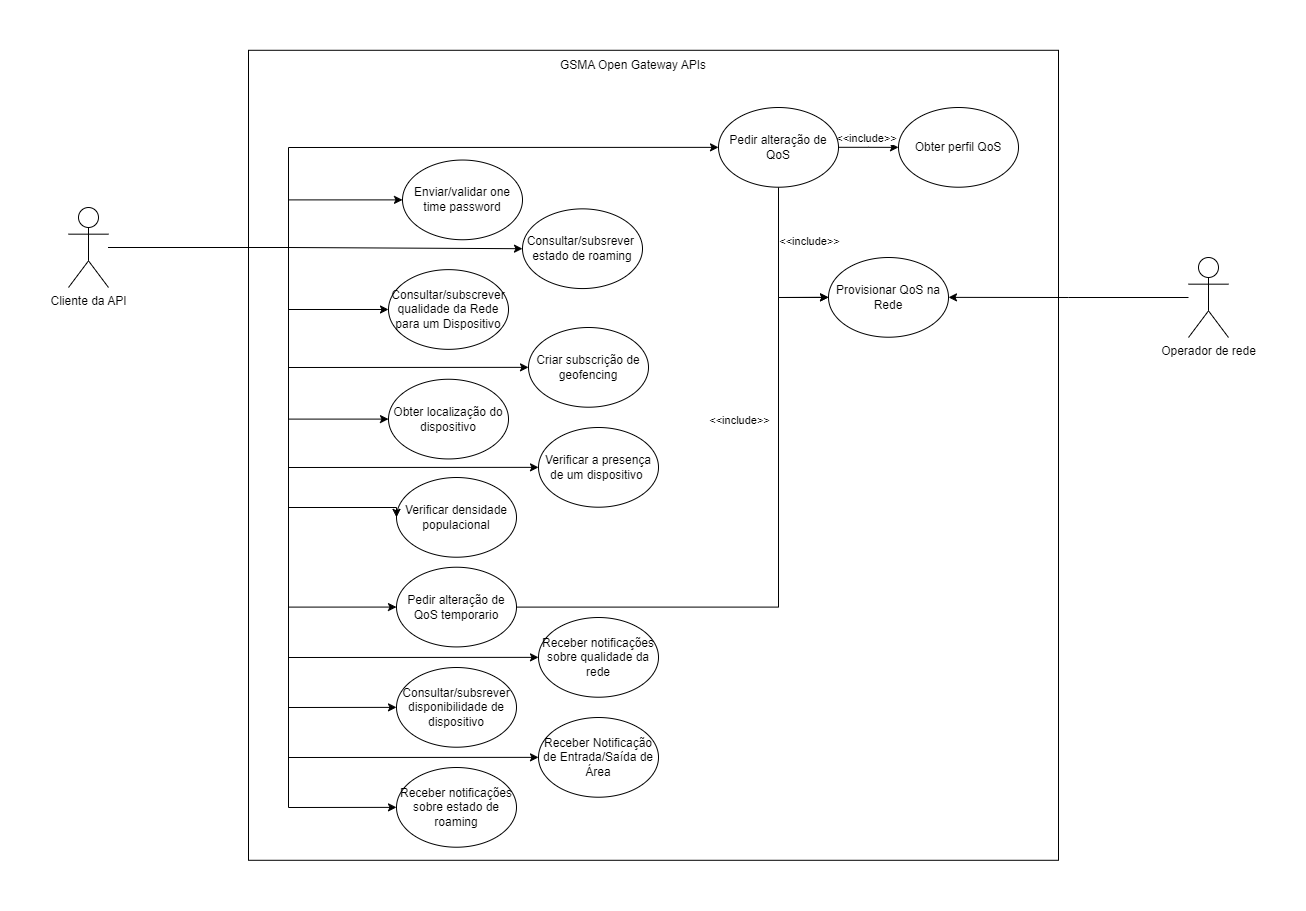
\includegraphics[width=20cm]{figs/use_case_diagram.png}
  }
  \caption{Use Case Diagram}
\end{figure}

\begin{itemize}
  \item \textbf{Network Operator}

    Although the network operator can interact directly with the \emph{5G
    core}, the network operator can use the APIs it makes available to more
    easily manage the quality of service of its network

  \item{\textbf{Vertical Clients}}

    The customers of the APIs are the various businesses that want to
    programmatically modify the network, either to offer better
    products/services to their customers, or to manipulate an internal network
    to better suit their needs. Using the APIs defined by the \emph{GSMA Open
    Gateway}, the various businesses can:
    \begin{enumerate}
      \item Send/Validate One Time Passwords (OTPs), to (for example) check the
        validity of a phone number via SMS

      \item Check or subscribe to roaming status, so you can verify whether 
        a device is in another country.

      \item Check and/or subscribe to the network quality for a given device,
        so that you know if the network requirements for the application can be
        met; if you subscribe, a notification will be sent whenever there is a
        change in quality.

      \item Obtain the location of a given device

      \item Check the presence of a device, i.e. check whether a particular
        device is within the defined area.

      \item Check the population density in a given area

      \item Request a QoS change, temporary or not, due to the need for more
        bandwidth.

      \item Receive notifications about network status

      \item Receive notifications regarding the entry or exit of a device from
        a given area

      \item Subscribe/Consult the availability of a device
    \end{enumerate}
\end{itemize}

\section{Requirements}

For the development of the system, the following requirements were gathered:

\subsection{Functional Requirements}

\begin{itemize}
  \item \textbf{Location Services:}
    \begin{itemize}

      \item The system must allow the creation of event subscriptions so that
        \emph{CAMARA API} clients receive notifications when they enter or leave a
        defined area.

      \item The system must make it possible to obtain the location of a
        device, this being described by a circle (coordinates of the center and
        radius) or a simple polygon (list of coordinates)

      \item The system must make it possible to check whether a device is in a
        certain area. If this area is outside the area covered by the operator
        or if this area is valid, among other things, it should return the
        correct errors.

      \item The system must make it possible to obtain an estimate of the
        population density in a specified area
    \end{itemize}

  \item \textbf{Communication Quality:}
    \begin{itemize}
      \item The system should allow the exchange of relevant information to help make
        decisions related to the network APIs.

      \item The system should allow developers to consult the network about the
        likelihood of meeting connectivity requirements in a session. 

      \item The system should allow developers to define different QoS on client APs,
        depending on their bandwidth needs.

      \item The system should allow the existing QoS profiles in a network to be
        obtained and the information relating to them to be returned.

      \item The system must allow QoS profiles to be assigned to a device. The
        network will apply the QoS profile to the device's traffic whenever it is
        connected, until this provisioning is removed.
    \end{itemize}

  \item \textbf{Fraud Protection:}
    \begin{itemize}
      \item The system must allow for the verification of a given phone number,
        through the emission and validation of an OTP.
    \end{itemize}

  \item \textbf{Device Information Gathering:}
    \begin{itemize}
      \item The system must make it possible to check whether a particular
        device is available on the network.

      \item The system must allow an API subscriber to be notified if there is
        a change in the availability of a particular device.

      \item The system must be able to check whether a particular device is
        roaming, and if so, return the existing information about the country.

      \item The system must allow an API subscriber to be notified if there is
        a change in the roaming status of a device.
    \end{itemize}
\end{itemize}

\subsection{Non-Functional Requirements}

\begin{itemize}
  \item \textbf{Performance and Latency:}
    \begin{itemize}
      \item The system should maintain consistent response times as the user base or data volume increases 

      \item The system must be able to handle an increasing number of requests.
    \end{itemize}

  \item \textbf{Scalability:}
    \begin{itemize}
      \item The system must ensure that the system supports a high volume of requests and connected devices

      \item The system must scale horizontally and/or vertically depending on demand.
    \end{itemize}

  \item \textbf{Availability and Reliability:}
    \begin{itemize} 
      \item The system must establish availability levels (e.g. 99.9\% SLA
        uptime) 

      \item The system must have a high level of reliability (i.e. 99.9999\%
        reliability)

      \item The system must have a redundancy and fault tolerance mechanism,
        guaranteeing continuous operation even under adverse conditions.
    \end{itemize}

  \item  \textbf{Interoperability:}
    \begin{itemize}
      \item The system must be compatible with different operators,
        guaranteeing the integration of APIs with the infrastructure of
        different network operators, promoting the universality of services.

      \item The system must ensure that APIs follow open standards and best
        practices, promoting interoperability and universal acceptance between
        different systems and technologies.
    \end{itemize}


  \item \textbf{Maintainability and Extensibility:}
    \begin{itemize}
      \item The system must have a modular architecture, allowing the system to
        be divided into independent components, facilitating updates and
        corrections without affecting the overall functioning.

      \item The system must have detailed documentation, with manuals, to help
        developers understand and maintain the system effectively.

      \item The system must have clean and readable code, following standards
        that make the code easy to understand and modify, reducing the
        likelihood of errors.

      \item The system should have flexibility for updates, making it easy to
        implement new features or improvements without having to rewrite large
        parts of the code.
    \end{itemize}

  \item \textbf{Usability:}
    \begin{itemize}
      \item The system should return errors, if any, following the defined
        standard, facilitating the integration of these APIs as well.

      \item The system should only return relevant information to the
        developer, abstracting them from more complex network information.
    \end{itemize}
\end{itemize}
